\documentclass[10pt,a4paper,oneside]{article}

% -------------------------------------------------------------
%             PACKAGES FROM THE J.UCS TEMPLATE
% -------------------------------------------------------------
\usepackage[hidelinks]{hyperref}      % already in your template
\usepackage{jucs2e}                   % the main J.UCS style
\usepackage{graphicx}
\usepackage{url}
\usepackage{ulem}
\usepackage{mathtools}
\usepackage{scalerel}
\usepackage{setspace}
\usepackage[strict]{changepage}
\usepackage{caption}
\usepackage[letterspace=-50]{microtype}
\usepackage{fontspec}
\usepackage{afterpage}
\usepackage{ragged2e}
\setmainfont{Times New Roman}
\usepackage{titlesec}
\titleformat*{\section}{\Large\bfseries}
\titleformat*{\subsection}{\normalsize\bfseries}
\renewcommand{\baselinestretch}{0.9} 
\graphicspath{{./figures/}}
\usepackage[textwidth=8cm, margin=0cm, left=4.6cm, right=4.2cm, top=3.9cm, bottom=6.8cm, a4paper, headheight=0.5cm, headsep=0.5cm]{geometry}
\usepackage{fancyhdr}
\usepackage[format=plain, labelfont=it, textfont=it, justification=centering]{caption}
\usepackage{breakcites}
\usepackage{microtype}
\apptocmd{\frame}{}{\justifying}{}
\urlstyle{same}
\pagestyle{fancy}

% -------------------------------------------------------------
%                  ADDITIONAL PACKAGES
% -------------------------------------------------------------
% If your paper uses algorithms, math, etc.:
\usepackage{amsmath}
\usepackage{algorithm}
\usepackage{algpseudocode}
\usepackage{xcolor}
\usepackage{longtable}
\usepackage{array}
\usepackage{booktabs}
\usepackage{placeins} % in your preamble

% etc., as needed

% -------------------------------------------------------------
%                HEADER DEFINITIONS (J.UCS)
% -------------------------------------------------------------
% \newcommand\jucs{{Journal of Universal Computer Science}}
% \newcommand\jucsvol{vol. 27, no. 1 (2021)}
% \newcommand\jucspages{2987-2989}
% \newcommand\jucssubmitted{1/1/2021}
% \newcommand\jucsaccepted{2/2/2021}
% \newcommand\jucsappeared{3/3/2021}
% \newcommand\jucslicence{CC BY-ND 4.0}
% \newcommand\startingPage{2987}
% \setcounter{page}{\startingPage}

% -------------------------------------------------------------
%                      PAPER-SPECIFIC
% -------------------------------------------------------------
\newcommand\paperauthor{{Tarkhanyan, A., Harutyunyan, A.: }}
\newcommand\papertitle{{\color{black}DSGD++: Reducing Uncertainty and Training Time in the DSGD Classifier through a Mass Assignment Function Initialization Technique}}

% Header content
% \header{\paperauthor \papertitle}

% -------------------------------------------------------------
%                  DOCUMENT BEGINS
% -------------------------------------------------------------
\begin{document}

% ------------------ TITLE AND AUTHORS ------------------------
\title{{\fontsize{14pt}{14pt}\selectfont{\vspace*{-3mm}\papertitle\vspace*{-1mm}}}}

\author{%
{\bfseries\fontsize{10pt}{10pt}\selectfont{Aik Tarkhanyan}} \\
{\fontsize{9pt}{12pt}\selectfont{Mathematics and Mechanics Department at Yerevan State University, 0025 Yerevan, Armenia\\
\orcid{0009-0000-7015-111X}, 
hayk.tarkhanyan@edu.ysu.am)}}
\and
{\bfseries\fontsize{10pt}{10pt}\selectfont{Ashot Harutyunyan}}\\
{\fontsize{9pt}{12pt}\selectfont{(ML Lab at Yerevan State University, 0025 Yerevan, Armenia, \\
Institute for Informatics and Automation Problems NAS RA, 0014 Yerevan, Armenia\\
\orcid{0000-0003-2707-1039},
harutyunyan.ashot@ysu.am)}}
}

\label{first}
\maketitle

% --------------------- ABSTRACT & KEYWORDS -------------------
{\fontfamily{ptm}\selectfont
\begin{abstract}
{\fontsize{9pt}{9pt}\selectfont{\vspace*{-2mm}
Several studies have shown that the Dempster–Shafer theory (DST) can be successfully applied to scenarios where model interpretability is essential. Although DST-based algorithms offer significant benefits, they face challenges in terms of efficiency. We present a method for the Dempster-Shafer Gradient Descent (DSGD) algorithm that significantly reduces training time—by a factor of 1.6—and also reduces the uncertainty of each rule (a condition on features leading to a class label)  by a factor of 2.1, while preserving accuracy comparable to other statistical classification techniques. Our main contribution is the introduction of a "confidence" level for each rule. Initially, we define the "representativeness" of a data point as the distance from its class's center. Afterward, each rule's \textit{confidence} is calculated based on \textit{representativeness} of data points it covers. This confidence is incorporated into the initialization of the corresponding Mass Assignment Function (MAF), providing a better starting point for the DSGD's optimizer and enabling faster, more effective convergence. The code is available at \url{https://github.com/HaykTarkhanyan/DSGD-Enhanced}.
}}
\end{abstract}
}

{\fontfamily{ptm}\selectfont
\begin{keywords}
{\fontsize{9pt}{9pt}\selectfont{
Dempster-Shafer Theory, Interpretability, KMeans, Mass Assignment Functions, Classification}}
\end{keywords}
}

% https://www.jucs.org/ujs/jucs/info/ACM_Categories.html
{\fontfamily{ptm}\selectfont
\begin{category}
{\fontsize{9pt}{9pt}\selectfont{
I.2.6, I.5, G.3
}}
\end{category}}

% {\fontfamily{ptm}\selectfont
% \begin{doi}
% {\fontsize{9pt}{9pt}\selectfont{
% 10.3897/jucs.\textless SubmissionNumber\textgreater}}
% \end{doi}}


% -------------------------------------------------------------
%                     MAIN BODY
% -------------------------------------------------------------

\section{Introduction}\label{sec1}
Dempster-Shafer theory \cite{dst} has emerged as a powerful framework for developing classification algorithms that prioritize interpretability. This theory provides a mathematical approach for combining evidence from different sources to calculate the probability of an event, utilizing Dempster's rule of combination. Peñafiel et al. \cite{sergio} have demonstrated {\color{black} for classification tasks} that an algorithm combining Dempster-Shafer theory with optimization techniques can offer substantial explainability, even when employing a limited number of rules, without sacrificing accuracy. {\color{black} The algorithm was further extended to the regression case by Baloian et al. \cite{Nelson} and to clustering by Valdivia et al. \cite{dsClustering}.}. The algorithm is inherently explainable because it operates by combining relatively simple rules for inference. {\color{black}Additionally, recent work by Baloyan et al \cite{Aneta} demonstrates {\color{black}the} algorithm's robustness to class imbalance and its ability to capture various numeric interactions {\color{black} among the individual properties (i.e., features) that define each data point.}}

To make improvements, two issues should be considered.  Firstly, the number of subsets in the frame of discernment, growing with a complexity of $\mathcal{O}(2^n)$, makes the inclusion of non-singleton classes nearly impossible. Secondly, given that each feature in the dataset typically generates three rules, combining even two rules significantly increases training time and further limits the predictive power of the rules. 
\textcolor{black}
{
Moreover, one promising direction for improving DST-based methods lies in incorporating rules derived from rule mining algorithms \cite{ripper, c5, skoperules}. However, to make this approach truly feasible, it becomes evident that a strategy to reduce training time is crucial for enhancing DST-based models.
}
% Added transition to next section for better flow
{\color{red}In the following section, we outline our methodology for addressing these challenges, focusing on improved Mass Assignment Function initialization to reduce training time and uncertainty.}
\section{Methodology}\label{1.2}
\subsection{Overview}\label{1.2.2}
Our approach significantly reduces the optimization time by improving the technique for initializing MAFs associated with the rules. Peñafiel et al. \cite{sergio} relied on random assignment, where the empty set's mass is set to 0, the entire set—which represents total uncertainty—is assigned a value of 0.8, and the remaining 0.2 is randomly distributed among singleton classes (other classes are not considered). {\color{black} Sedláček et al. \cite{czechs} have investigated the use of the statistical distribution of classes in allocating mass values}. Here{\color{black},} we propose a {\color{black} clustering-based} technique that incorporates additional information about each rule into the MAF. 

To advance this method, we introduce the concept of rule "confidence". First of all, operating under the assumption that certain points are more representative of their class than others{\color{black},} we define "representativeness" for each point. This approach is inspired by the post-hoc interpretation technique commonly used in clustering algorithms. In these models, each cluster's "color" is treated as a label, upon which interpretable classifiers are constructed. In our framework, we not only assign a "color" to data points{\color{black},} but also attribute a numeric value representing their "opacity" which we refer to as "representativeness". For spherical data, we employ the $get\_representativeness\_KMeans$ function (see Algorithm \ref{alg:representativeness_kmeans}), which uses the KMeans clustering algorithm \cite{kmeans} to determine the most representative data point. {\color{black}In our previous work (\cite{menq}) we were simply setting the most representative data point to the arithmetic mean of the data points with the same label instead of using KMeans.} In scenarios where data is better suited for density-based clustering, we apply the $get\_representativenes\_DBSCAN$ function (see Algorithm \ref{alg:representativeness_DBSCAN}, {\color{black}which is based on DBSCAN \cite{DBSCAN} algorithm.} Once we have determined the representativeness of each data point, we then define the confidence of each rule of the data points following that rule, this is achieved by $get\_confidence$ function discussed in Section \ref{2.3}. The final step involves integrating this confidence into the MAF assignment, which will be discussed further in Section \ref{2.4}.

% Added roadmap for methodology subsections
{\color{red}The remainder of this section is structured as follows: Section~\ref{1.2.1} describes representativeness estimation, Section~\ref{2.3} covers rule confidence computation, and Section~\ref{2.4} details the enhanced MAF initialization.}
\subsection{Estimation of Representativeness}\label{1.2.1}
Below, we present the algorithms for estimation of representativeness using KMeans clustering (Algorithm \ref{alg:representativeness_kmeans}) and the DBSCAN-based (Algorithm \ref{alg:representativeness_DBSCAN}) approaches. Additionally, we present example figures for synthetic datasets (Figure \ref{fig:reprs}).

In the \textbf{KMeans-based approach}, the data is standardized and then clustered into \(k\) groups (same as the number of classes). Each data point’s representativeness is determined by its distance to the cluster centroid: points are first checked for outlier status using a Z-score threshold, and then distances are normalized within each cluster. The representativeness score is calculated as \(1\) minus the normalized distance (or \(0\) if the point is flagged as an outlier).

In the \textbf{DBSCAN-based approach}, the algorithm begins with a small initial neighborhood radius (e.g., \(\varepsilon = 0.1\)) and then increases this radius in small increments until it either reaches \textit{maxEps} or yields the desired number of clusters. After each increment, DBSCAN is applied, and the resulting number of clusters is checked against the target \(k\). If there are too few clusters, \(\varepsilon\) is incremented further, leading to larger neighborhoods and fewer clusters merging. Once a specific \(\varepsilon\) value produces the target number of clusters, each data point’s representativeness is computed by counting how many points fall within that final radius, and these counts are then scaled via Min-Max normalization.

\textbf{Note:} The following hyperparameters are used:
\begin{enumerate}
    \item KMeans-based approach: $zScoreThreshold = 2$
    \item DBSCAN-based approach: $minPoints = 2 \times (\text{number of features})$; $maxEps = 20$; $step = 0.05$ 
\end{enumerate}

\begin{algorithm}
\caption{Estimation of Representativeness using KMeans Clustering}
\label{alg:representativeness_kmeans}
\begin{algorithmic}[1]
\Require $X$: Dataset, $k$: Number of clusters (same as dataset's number of classes), 
\Ensure $representativenessList$: List of representativeness values for each data point
\Function{get\_representativeness\_KMeans}{$X$, $k$}

\State Standardize the dataset $X$ using standard scaling.
\State Fit the KMeans clustering algorithm on $X$ with $k$ clusters to obtain centroids $\{C_i\}_{i=0}^{k-1}$.
\State $confidenceList \gets$ Empty list
\For{each $dataPoint$ in $X$}
    \State Calculate Euclidean distance from $dataPoint$ to its nearest centroid $C_i$.
\EndFor
\State Identify outliers among the data points using the Z-score technique, where a data point is considered an outlier if its distance's Z-score exceeds $zScoreThreshold$.
    \If{$dataPoint$ is not an outlier}
        \State $normalizedrepresentativeness \gets dataPoint$'s distance after normalizing using min-max scaling within its cluster.
        \State $representativeness \gets 1 - normalizedrepresentativeness$
    \Else
        \State $representativeness \gets 0$
    \State Append $representativeness$ to $representativenessList$
    \EndIf
\EndFor
\State \Return $representativenessList$
\EndFunction
\end{algorithmic}
\end{algorithm}


\begin{algorithm}
\caption{Estimation of Representativeness using Density Based Approach}
\label{alg:representativeness_DBSCAN}
\begin{algorithmic}[1]
\Require $X$: Dataset, $k$: Number of clusters (same as number of unique classes), \Ensure $confidenceList$: List of confidence scores for each data point
\Function{get\_representativeness\_DBSCAN}{$X$, $k$}
\State Standardize the dataset $X$ using standard scaling.
\State Initialize $eps \gets$ Initial small value (e.g., 0.1)
\While{$numCentroids \neq k$ and $eps \leq maxEps$}
    \State $model \gets$ DBSCAN($eps$, $minPoints$)
    \State Fit DBSCAN on $X$
    \State $numCentroids \gets$ Count of unique clusters formed (excluding noise)
    \State $eps \gets eps + step$
\EndWhile
\State $radius \gets eps$
\State Initialize $confidenceList \gets$ Empty list
\For{each $dataPoint$ in $X$}
    \State $representativeness \gets \sum\limits_{y \in X} \mathbf{1}_{\|y - x\| \leq radius}$ (number of data points within the specified radius)
    \State Append $representativeness$ to $representativenessList$
\EndFor
\State $representativenessList \gets$ Min-Max Scaled version of $representativenessList$ 
\State \Return $representativenessList$
\EndFunction
\end{algorithmic}
\end{algorithm}

\begin{figure}[H]
    \centering
    \begin{minipage}{0.49\textwidth}
        \includegraphics[width=\linewidth]{figures/kmeans_opactiy.png} % First image
    \end{minipage}\hfill
    \begin{minipage}{0.49\textwidth}
        \includegraphics[width=\linewidth]{figures/denisty_opactiy.png} % Second image
    \end{minipage}
    \caption{Illustrations of algorithms for estimation of representativeness for datasets with spherical shapes and density-based characteristics. Brighter colors indicate data points that are more representative of their respective classes.}
    \label{fig:reprs}
\end{figure}

Our next step is aggregating the representativeness values for data points that follow the same rule into a measure of rule confidence.

% \newpage
\subsection{Rule Confidence Estimation}\label{2.3}
Utilizing the algorithms previously described, we calculate the representativeness for each data point. Afterward, we generalize this data point-specific estimate to an entire rule using the following steps (we encapsulate this in the $get\_confidence$ function):
\begin{enumerate}
    \item Filter the dataset to retain only the rows that comply with the rule.
    \item If the rule does not apply to any rows, set its confidence to 0 (this corresponds to the full uncertainty). Otherwise:
    \item Calculate the rule's confidence as the mean representativeness of the rows it covers.
    \item If the rows are not homogeneous with respect to their labels, reduce the confidence based on the proportion of the most frequent label among these rows.
\end{enumerate}

Once we have obtained the confidence scores for the rules we can incorporate them into the MAF initialization.

\subsection{MAF Initialization}\label{2.4}
In the MAF, we use the following values for initialization. Let $c = get\_confidence(rule)$ represent the confidence derived for a given rule. The label $l_{\text{mode}}$, which is the most frequently occurring label within the subset of data points covered by the rule, receives the confidence value $c$. The remaining mass, $(1 - c)$, is evenly distributed among all the other labels present in the subset. Formally, for an element $l_i$ in the subset:
\[
m(l_i) = 
\begin{cases} 
c & \text{if } l_i = l_{\text{mode}}, \\
\frac{1-c}{n-1} & \text{otherwise},
\end{cases}
\]
where $m(l_i)$ denotes the mass assigned to label $l_i$, and $n$ is the total number of elements in the frame of discernment. Note that here by saying label we mean the original label of the data point, not the one assigned to it via clustering algorithm (the color). 

% Smoother transition to Results section
{\color{red}In the following section, we compare the results of initializing MAFs with the proposed approach and the traditional random initialization.}

\section{Results}
Here{\color{black},} we demonstrate the effects of the newly defined MAF initialization algorithm (KMeans-based) on the training time, accuracy, and the amount of rule uncertainties. We accomplish this by testing the approach both on controlled scenarios and on some classical datasets. The datasets used for evaluations are summarized in Table \ref{datasets}. 
\\
\begin{longtable}{|>{\raggedright\arraybackslash}p{3cm}|c|c|>
{\raggedright\arraybackslash}p{5cm}|}
\caption{Datasets overview (binary classification)}
\label{datasets}
\\
\hline
\textbf{Dataset} & \textbf{Rows} & \textbf{Columns} & \textbf{Description} \\ \hline
\endfirsthead
\hline
\textbf{Dataset} & \textbf{Rows} & \textbf{Columns} & \textbf{Description} \\ \hline
\endhead
Brain Tumor & 3762 & 14 & Includes first-order and texture features with target levels. \\ \hline
Breast Cancer Wisconsin & 699 & 9 & Clinical reports detailing cell benignity or malignancy. \\ \hline
Gaussian & 500 & 3 & Two 2D Gaussian distributions generate this dataset. \\ \hline
Uniform & 500 & 3 & Uniform samples from [-5, 5], with class split by the sign of x. \\ \hline
Rectangle & 1263 & 3 & Points in [-1, 1]×[-1, 1], class determined by the y component's sign. \\ \hline

\end{longtable}
The first two are real-life datasets (\cite{breastCancer,brainTumor}), while the last three are controlled scenarios.

% Smoother transition to analysis subsections
{\color{red}The following subsections detail our findings: Section~\ref{sec:accuracy-speedup} presents accuracy and speedup results, and Section~\ref{sec:uncertainty-analysis} covers uncertainty analysis (we also do an evaluation of our newly proposed definition of uncertainty)}.

\subsection{Accuracy and Speedup Analysis}\label{sec:accuracy-speedup}
In this subsection, we focus on the KMeans approach, which we will refer to as the "clustering" MAF method. Additionally, we will use "MED." to denote the median and "AVG." to denote the average.

Table \ref{comparison} presents a comparison of various metrics across different MAF initialization methods (Confidence and Random) and datasets. For evaluating the classifier's predictive power, we have calculated the accuracy (ratio of correctly predicted instances to the total instances) and F1 score. For evaluating the optimizer, we have reported the training time in seconds, the number of epochs, the minimum loss, and the initial loss.

\begin{table}[H]
    \centering
    \caption{Comparison of various metrics across different MAF initializations and datasets}
    \label{comparison}
    \begin{tabular}{l|l|r|r|r|r|r|r}
    \toprule
    MAF method & dataset & accuracy & f1 & training\_time & epochs & min\_loss & initial\_loss\\
    \midrule
    clustering & Brain Tumor & 0.981 & 0.98 & 138.469 & 117 & 0.018 & 0.181 \\
    random & Brain Tumor & 0.983 & 0.981 & 157.075 & 132 & 0.026 & 0.245 \\
    clustering & Breast Cancer & 0.976 & 0.966 & 17.243 & 73 & 0.023 & 0.228 \\
    random & Breast Cancer & 0.976 & 0.966 & 19.63 & 117 & 0.031 & 0.308 \\
    clustering & Gaussian & 0.987 & 0.988 & 15.792 & 100 & 0.017 & 0.083 \\
    random & Gaussian & 0.987 & 0.988 & 39.059 & 264 & 0.024 & 0.265 \\
    clustering & Rectangle & 1 & 1 & 61.032 & 167 & 0.006 & 0.252  \\
    random & Rectangle & 1 & 1 & 98.64 & 275 & 0.008 & 0.235 \\
    clustering & Uniform & 0.973 & 0.97 & 20.683 & 120 & 0.035 & 0.197  \\
    random & Uniform & 0.973 & 0.97 & 39.208 & 273 & 0.037 & 0.255 \\
        \bottomrule
    \end{tabular}
\end{table}

% \newpage
We can see that our method requires fewer epochs to converge in all the cases, not only that, it also starts from a better point and converges to a smaller loss.

\FloatBarrier

\begin{figure}[htbp]
    \centering
    \label{talbe-ratios}
    \begin{minipage}{0.49\textwidth}
        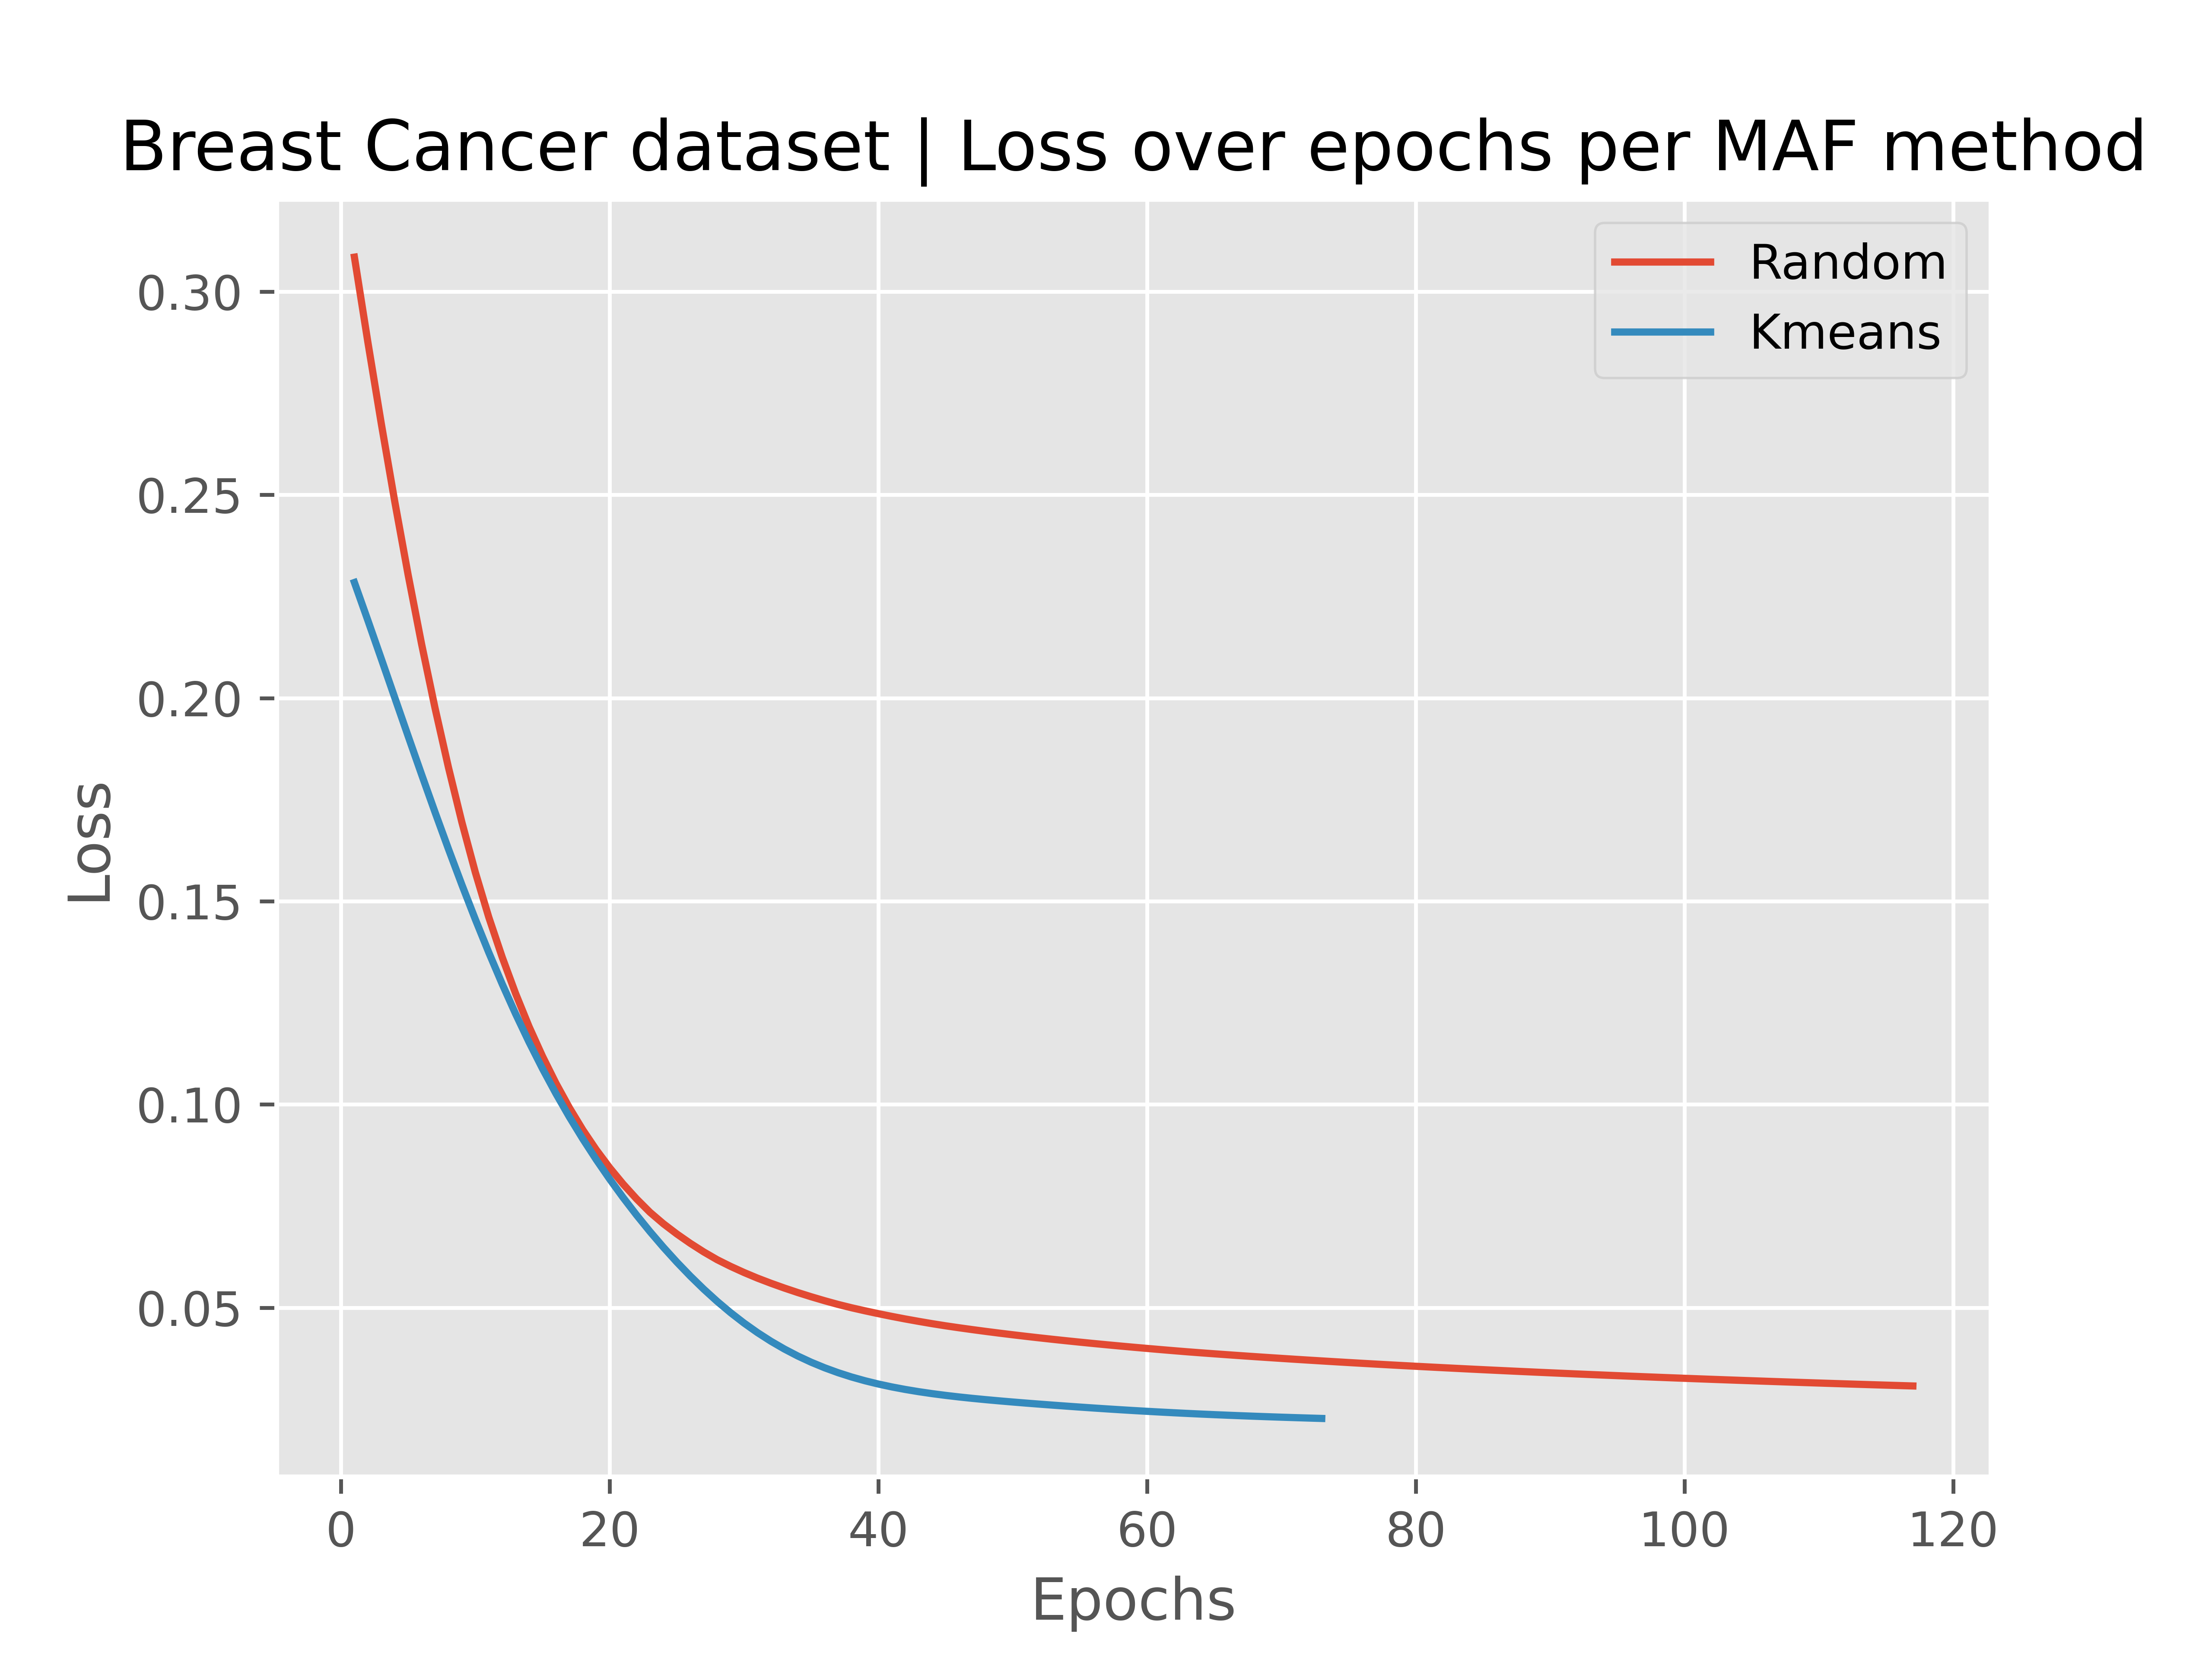
\includegraphics[width=\linewidth]{figures/breast-cancer-wisconsin_loss.png} % First image
    \end{minipage}\hfill
    \begin{minipage}{0.49\textwidth}
        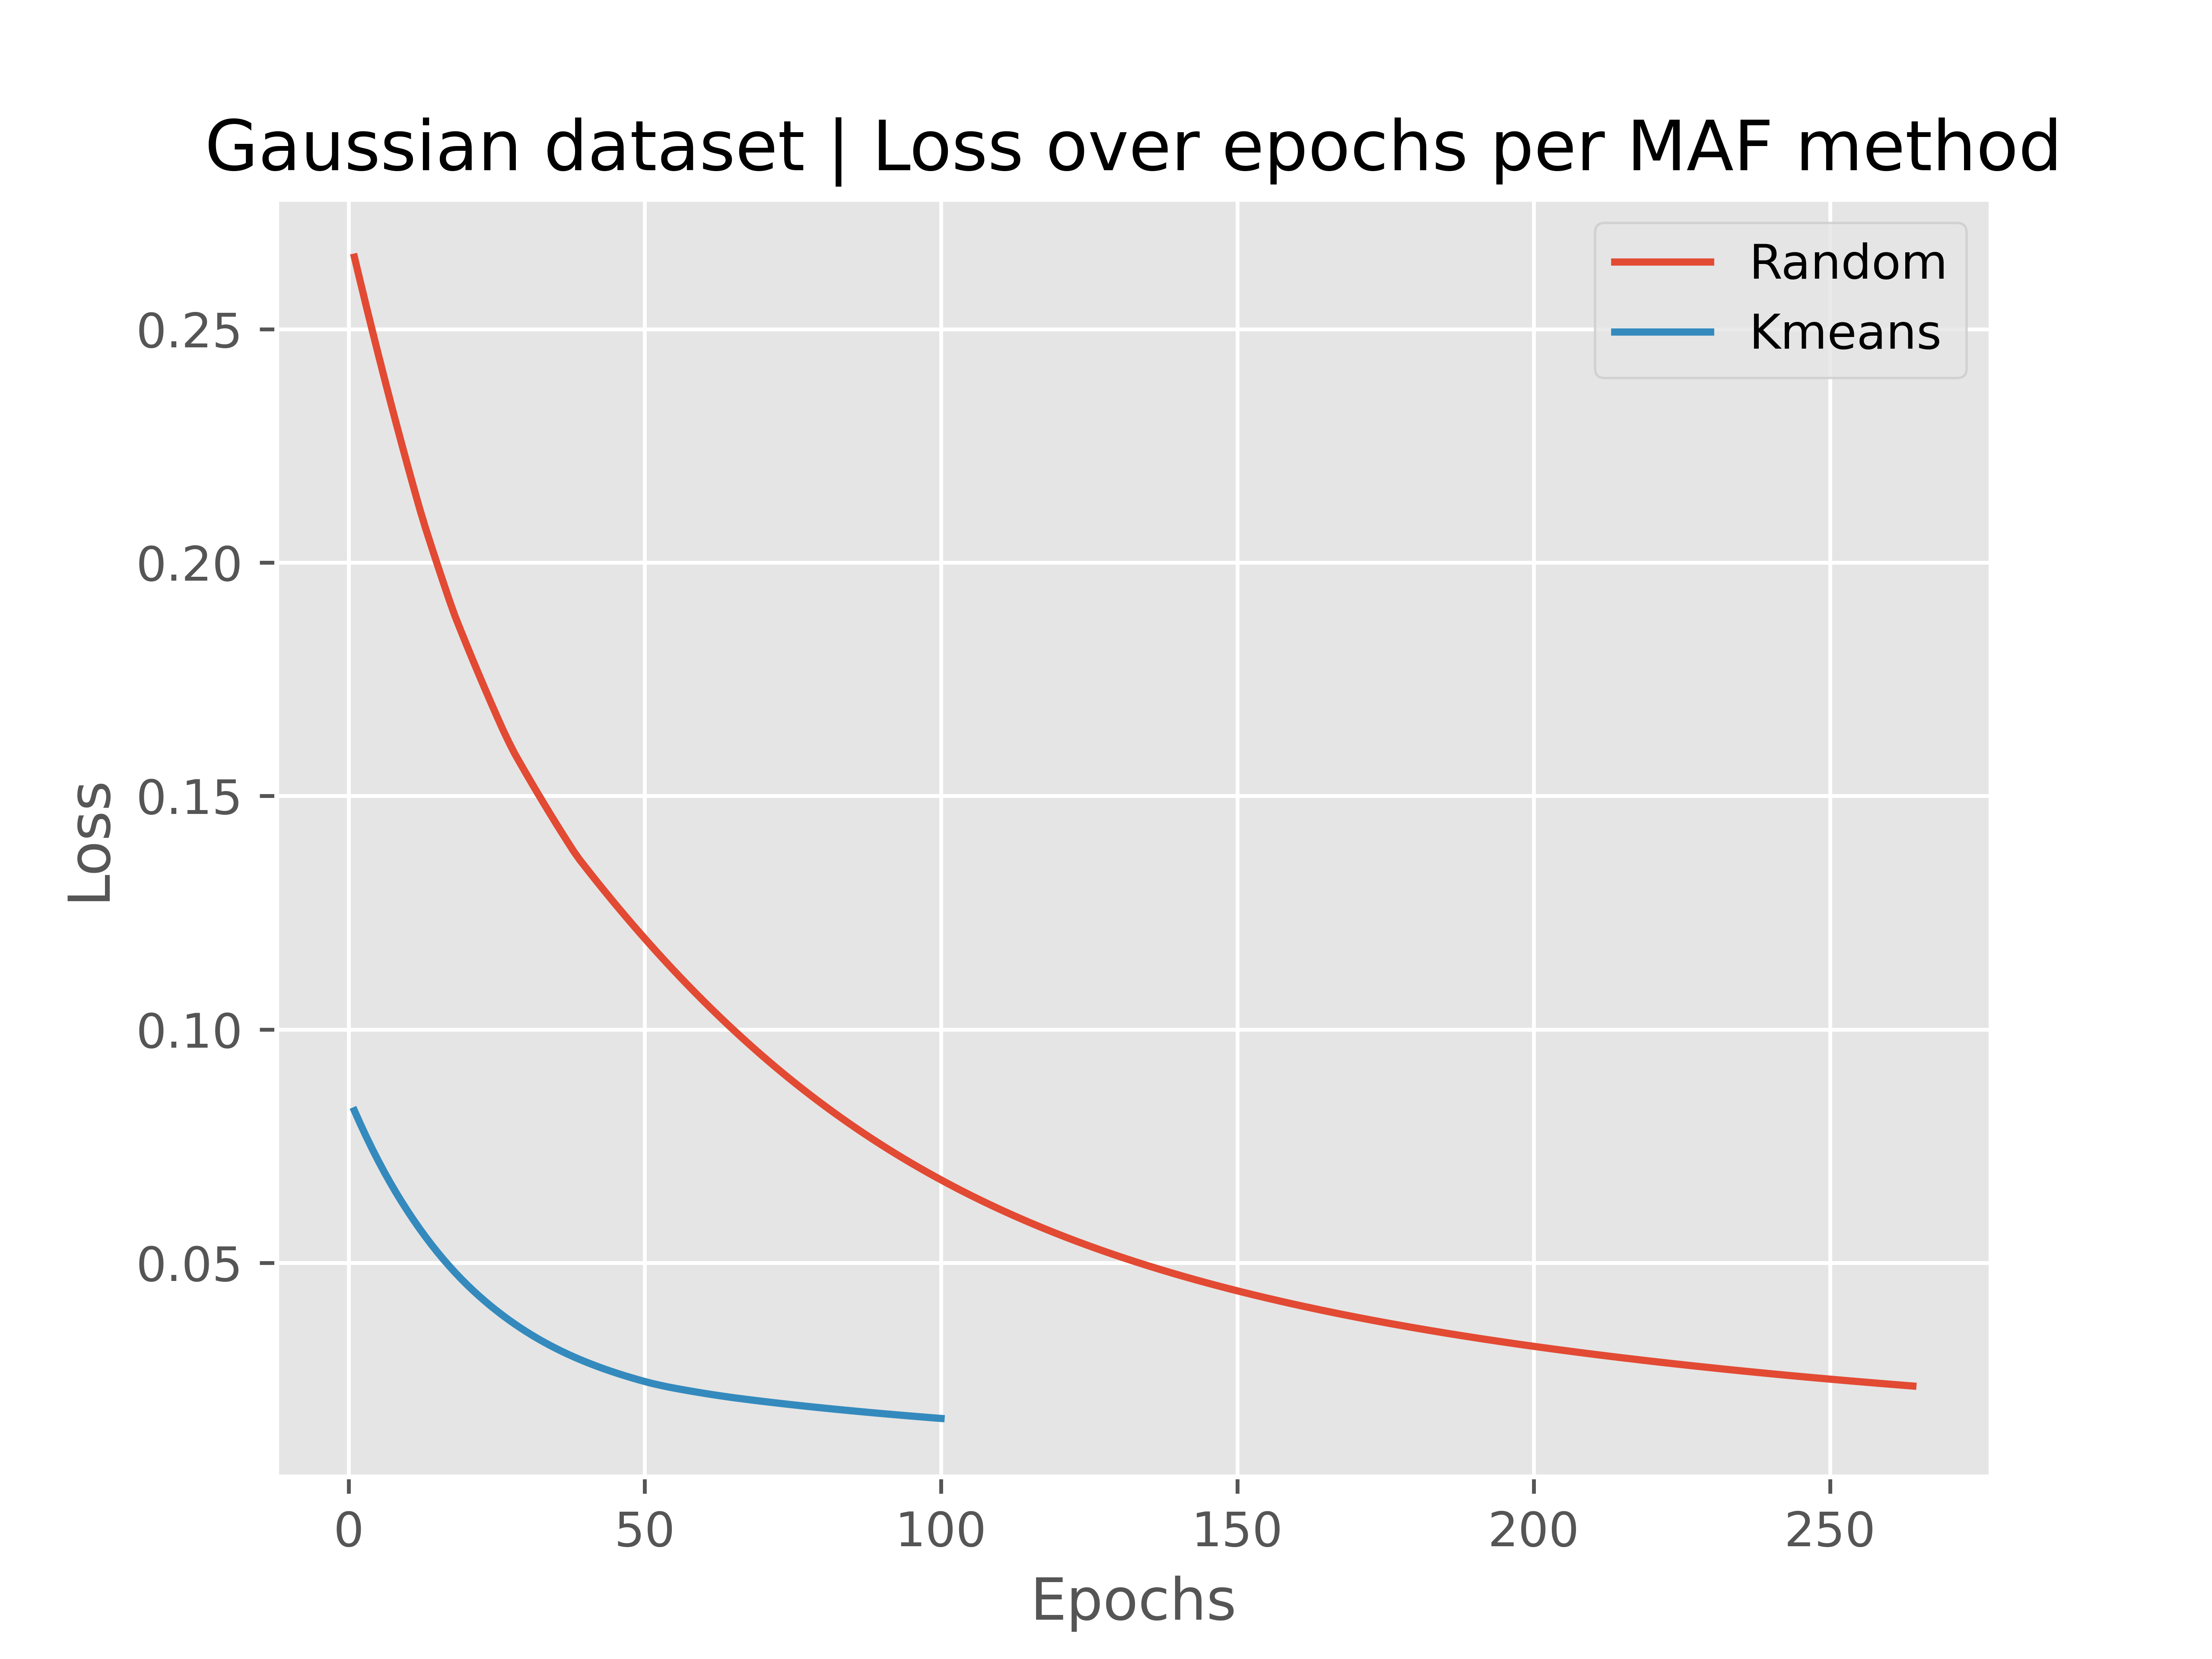
\includegraphics[width=\linewidth]{figures/gaussian_df_loss.png} % Second image
    \end{minipage}
    \caption{The figure demonstrates the benefits offered by MAF initialization, mainly decreased number of epochs and better starting point.}
    \label{fig:side_by_side}
\end{figure}

\newpage
Table \ref{table-ratios} deals with the speedup and predictive performance tradeoff. \\

\begin{table}[htbp]
    \centering
    \caption{Ratios of accuracy, F1 score, and training time for Random and Confidence MAF initializations across datasets}
    \label{table-ratios}
    \begin{tabular}{l|r|r|r}
    \toprule
    Dataset & Accuracy Ratio & F1 Ratio & Training Time Speedup, x \\
    \midrule
Brain Tumor & 1 & 1 & 1.13 \\
Breast Cancer & 1 & 1 & 1.14 \\
Gaussian & 1 & 1 & 2.47 \\
Rectangle & 1 & 1 & 1.62 \\
Uniform & 1 & 1 & 1.90 \\
    \bottomrule
    \end{tabular} \\
\end{table}

The results in Table \ref{table-ratios} were rounded up to 2 digits. We can infer that accuracy and the f1 score remain unchanged while we experience a speedup of 1.65x.


\subsection{Uncertainty Analysis}\label{sec:uncertainty-analysis}
After the model has been trained, the question arises of how reliable the rules used by the model are. To determine this, we must examine the MAFs associated with these rules. In this subsection, we will describe the traditional definition of uncertainty, demonstrate its weaknesses, suggest an alternative definition, and analyze both traditional and newly suggested uncertainties for different MAF initialization methods.

\subsubsection{A New Approach to Rule Importance Estimation}
Traditionally, uncertainty has been defined by the mass of the complete set, with lower uncertainty indicating a more reliable rule. However, this is not always the best approach. Table \ref{table-pitfalls} demonstrates an example. 

\begin{table}[ht]
    \centering
    \caption{Illustration of the Pitfalls of the Traditional Approach}
    \label{table-pitfalls}
    \begin{tabular}{c|c|c|c|c}
        \toprule
        \textbf{Rule} & \textbf{Mass First Class} & \textbf{Mass Second Class} & \textbf{Uncertainty} & \textbf{Ratio} \\
        \midrule
        1 & 0.49 & 0.51 & 0 & 1.04 \\
        2 & 0.01 & 0.09 & 0.9 & 9 \\
        \bottomrule
    \end{tabular}

\end{table}
Rule 1 shows zero uncertainty, which might seem ideal. But the nearly equal masses for the two classes make it hard for the algorithm to distinguish between them. On the flip side, Rule 2, despite its high uncertainty, has a significant difference in class masses (a ratio of 9), which enhances its ability to clearly separate the classes.

Given these insights, we propose a fresh approach that factors in both the uncertainty and the ratio between the most probable and second most probable masses.

Our method is inspired by the F1 score, which is the harmonic mean of precision and recall. To optimize our evaluation, we focus on maximizing the value of $1 - \textit{uncertainty}$ and the class mass \textit{ratio}. This approach allows us to prioritize both a high ratio and low uncertainty simultaneously. To unify these metrics into a single measure, we calculate their harmonic mean. However, since 1 - \textit{uncertainty} ranges from 0 to 1 and the \textit{ratio} can vary widely, we first normalize the \textit{ratio} using min-max scaling across all rules before applying the harmonic mean. This scaling ensures that both metrics contribute equally to the final score.
To put this formally 
\begin{itemize}
    \item \textbf{Uncertainty Adjustment:}
    \[
    U' = 1 - U
    \]
    where \( U \) is the original uncertainty.

    \item \textbf{Normalization of the Ratio:}
    \[
    R' = \frac{R - \min(R)}{\max(R) - \min(R)}
    \]
    where \( R \) is the original ratio (when dividing the values of two masses we add $\varepsilon=0.01$ to denominator to avoid zero division error), and \( \min(R) \) and \( \max(R) \) are the minimum and maximum values of the ratio across all rules, respectively.

    \item \textbf{Harmonic Mean Calculation:}
    \[
    H = \frac{2 \cdot U' \cdot R'}{U' + R'}
    \]
    where \( U' \) is the adjusted uncertainty value and \( R' \) is the normalized ratio.
\end{itemize}

% Transition to experimental results
{\color{red}With these definitions in place, we now present the experimental evaluation of both the traditional and proposed uncertainty measures.}

\subsubsection{Experimental Results}
Now we'll take a look at the effect of our new MAF initialization both based on traditional approach for importance calculation, and on newly proposed one. Below, we will define improvement as the ratio of $MED. Random$ and $MED. Clustering$.

\FloatBarrier

\begin{table}[htbp]
    \caption{Average and median uncertainties for Random and Clustering MAF initializations}
    \centering
    \label{unc-res}
    \begin{tabular}{l|r|r|r|r|r}
    \toprule
    Dataset & AVG. Clust. & AVG. Rand. & Med. Clust. & Med. Rand. & Improvement \\
    \midrule
    Brain Tumor & 0.258 & 0.713 & 0.246 & 0.732 & 2.979 \\
    Breast Cancer & 0.314 & 0.710 & 0.262 & 0.703 & 2.685 \\
    Gaussian & 0.225 & 0.330 & 0.229 & 0.302 & 1.318 \\
    Rectangle & 0.201 & 0.448 & 0.203 & 0.434 & 2.135 \\
    Uniform & 0.150 & 0.262 & 0.096 & 0.144 & 1.493 \\
    \bottomrule
    \end{tabular}
\end{table}
 Table \ref{unc-res} shows that on average the clustering approach yields in uncertainty reduction by a factor of 2.12.

\newpage
\FloatBarrier
\begin{table}[htbp]
    \caption{Average and median newly defined uncertainties for Random and Clustering MAF initializations}
    \centering
    \label{new-unce-res}
    \begin{tabular}{l|r|r|r|r|r}
    \toprule
    Dataset & AVG. Clust. & AVG. Rand. & Med. Clust. & Med. Rand. & Improvement \\
    \midrule
    Brain Tumor & 0.247 & 0.313 & 0.075 & 0.336 & 4.471 \\
    Breast Cancer & 0.156 & 0.359 & 0.075 & 0.411 & 5.486 \\
    Gaussian & 0.633 & 0.625 & 0.807 & 0.757 & 0.937 \\
    Rectangle & 0.473 & 0.536 & 0.457 & 0.571 & 1.249 \\
    Uniform & 0.732 & 0.700 & 0.935 & 0.876 & 0.937 \\
    \bottomrule
    \end{tabular}
    \label{tab:my_label}
\end{table}

Table \ref{new-unce-res} shows that on average the clustering approach yields in uncertainty reduction (harmonic mean approach) by a factor of 2.61.

{\color{black}
See below Figure \ref{fig:bars} for an example of rule uncertainties for the Breast Cancer dataset \cite{breastCancer}.
}
\FloatBarrier
\begin{figure}[htbp]
    \makebox[\textwidth][c]{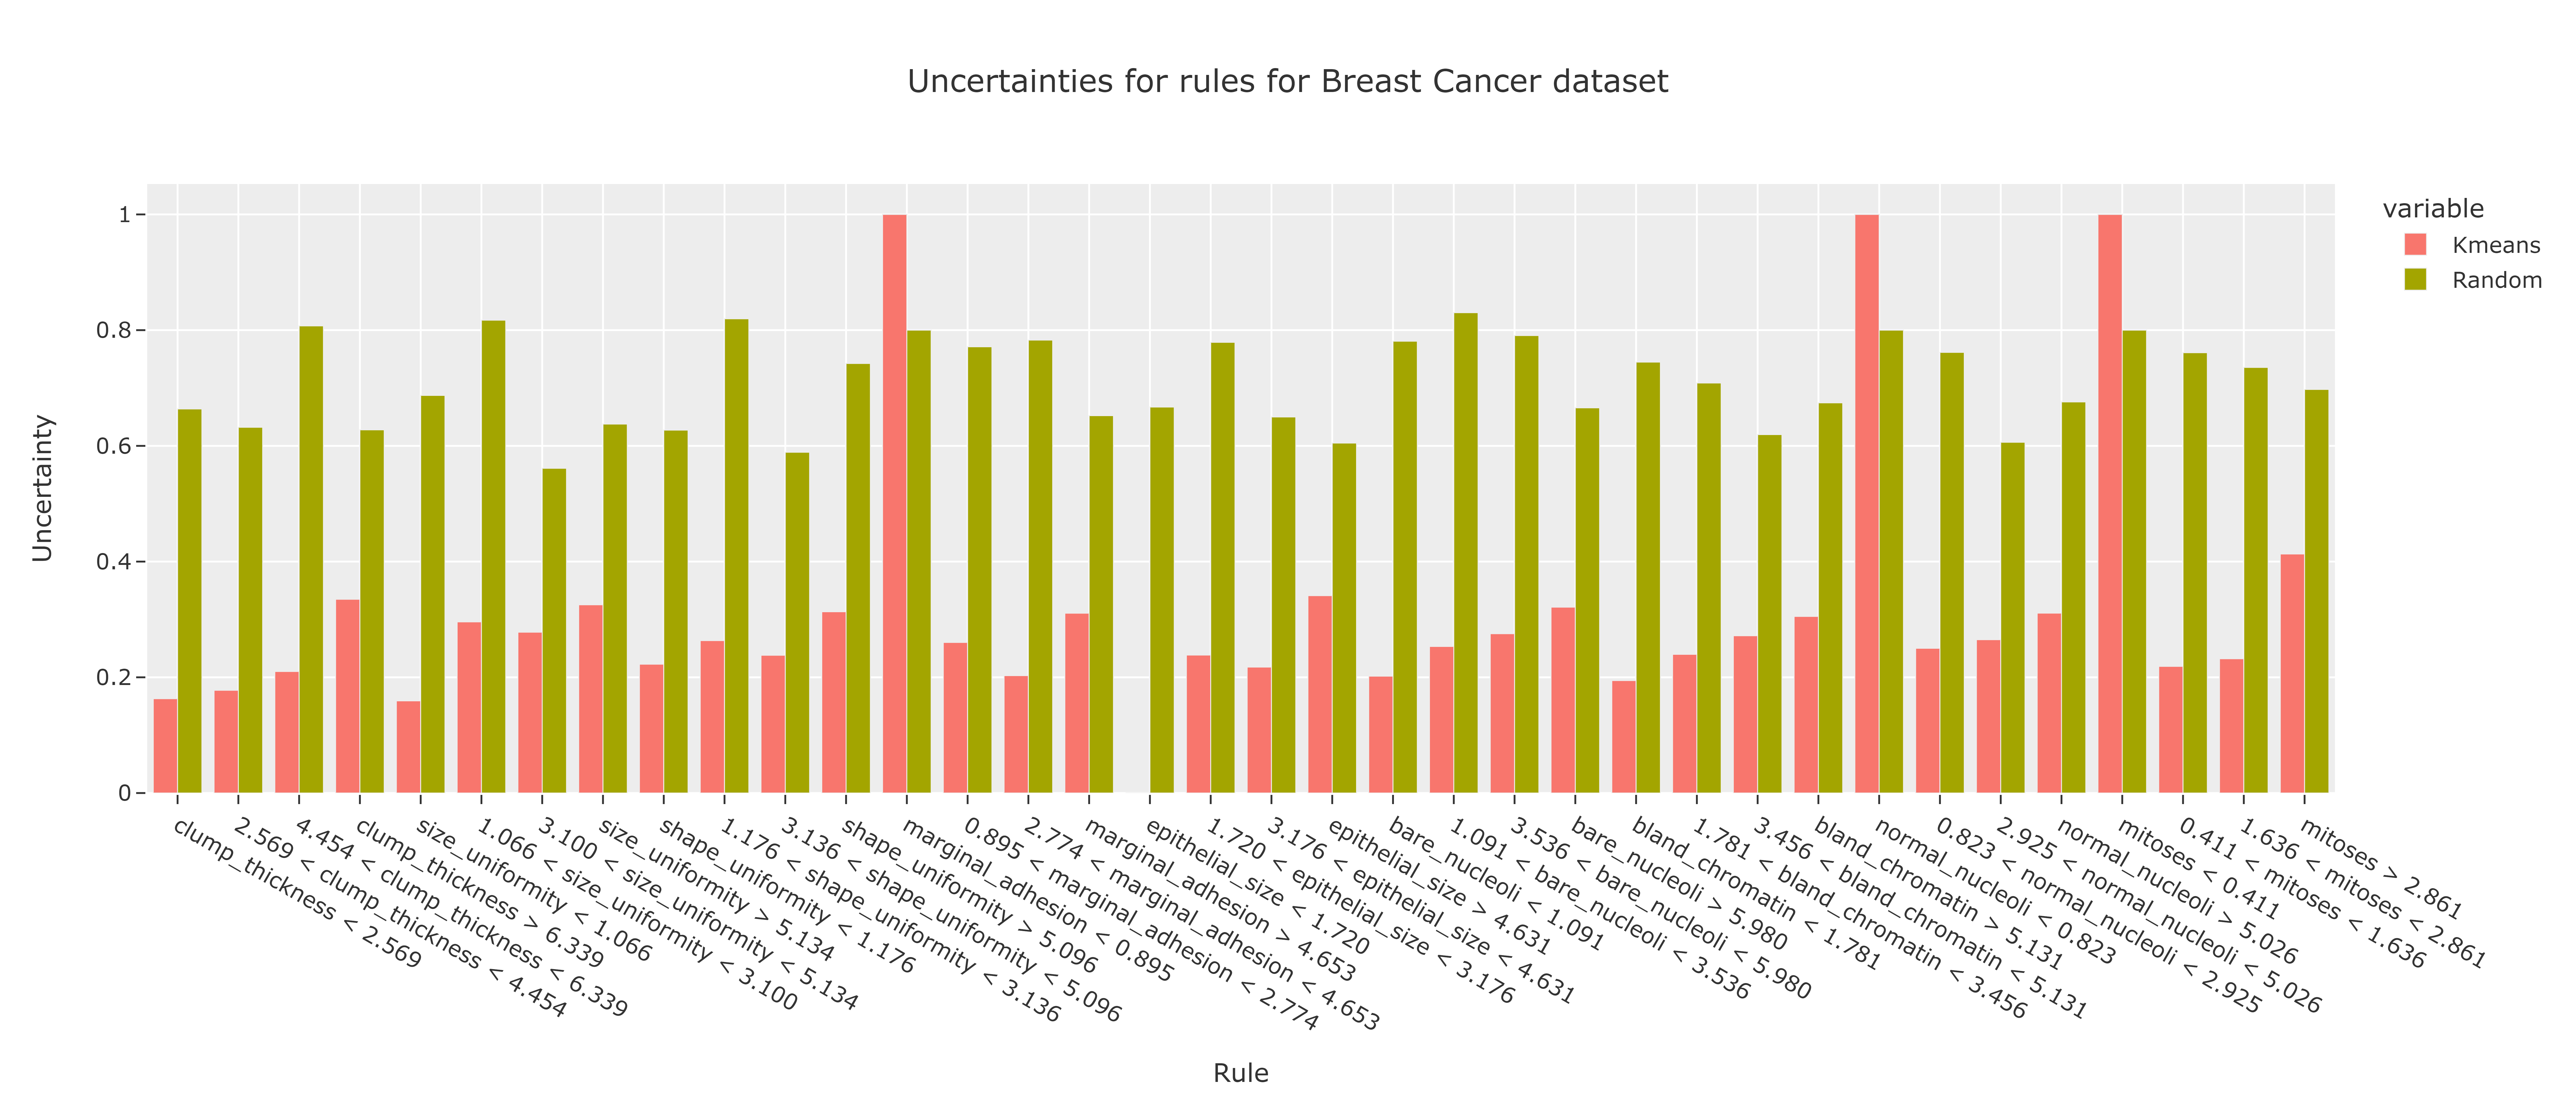
\includegraphics[width=0.9\linewidth]{figures/bars.png}} 
    \caption{Uncertainties per rule for different MAF initialization methods}
    \label{fig:bars}
\end{figure}


\section{Conclusions and Future Work}
We saw that by introducing the concept of \textit{representativeness} for individual data points—and using it to guide clustering-based MAF initialization—we achieved a 1.6× reduction in training time for DSGD classifier. The proposed initialization method not only offers a more favorable starting point for optimization{\color{black},} but also reduces the number of required epochs, all while preserving predictive performance equivalent to baseline method.

We further addressed the need for a more flexible definition of rule uncertainty by proposing a measure that takes into account the ratio of masses of singleton classes. Our MAF initialization approach reduced uncertainty by a factor of 2.6 using the newly proposed measure and by 2.1 using the traditional measure.

Future work may involve extending this approach to multi-label datasets, exploring additional clustering techniques, and leveraging the reduced training time to incorporate non-singleton classes or increase the number of generated rules.


% -------------------------------------------------------------
%              ACKNOWLEDGEMENTS (J.UCS)
% -------------------------------------------------------------
\begin{Acknowledgements}
The research was supported by ADVANCE Research Grants from the Foundation for Armenian Science and Technology.
\end{Acknowledgements}

% -------------------------------------------------------------
%                    REFERENCES (J.UCS)
% -------------------------------------------------------------
\begin{thebibliography}{}{
\fontsize{9pt}{10pt}\selectfont
\bibitem[Shafer, 76]{dst}
Shafer, G.: "A Mathematical Theory of Evidence";
Princeton University Press, Princeton (1976).

\bibitem[Peñafiel, 20]{sergio}
Peñafiel, S., Baloian, N., Sanson, H., Pino, J.A.: "Applying Dempster–Shafer Theory for Developing a Flexible, Accurate and Interpretable Classifier";
Expert Systems with Applications, 148 (2020), 113262.

\bibitem[Baloian, 24]{Nelson}
Baloian, N., Davtyan, E., Petrosyan, K., Poghosyan, A., Harutyunyan, A., Penafiel, S.:
"Embedded Interpretable Regression using Dempster-Shafer Theory";
In: Proceedings of the 4th Codassca Workshop on Data Science and Reliable Machine Learning (2024).

\bibitem[Valdivia, 24]{dsClustering}
Valdivia, R., Baloian, N., Chahverdian, M., Adamyan, A., Harutyunyan, A.:
"An Explainable Clustering Algorithm using Dempster-Shafer Theory";
In: Proceedings of the 4th Codassca Workshop on Data Science and Reliable Machine Learning (2024).

\bibitem[Baloyan, 24]{Aneta}
Baloyan, A., Aramyan, A., Baloian, N., Poghosyan, A., Harutyunyan, A., Penafiel, S.:
"An Empirical Analysis of Feature Engineering for Dempster-Shafer Classifier as a Rule Validator";
In: Proceedings of the 4th Codassca Workshop on Data Science and Reliable Machine Learning (2024).

\bibitem[Cohen, 95]{ripper}
Cohen, W.W.: "Fast Effective Rule Induction";
In: Prieditis, A., Russell, S. (eds.) Machine Learning Proceedings 1995,
Morgan Kaufmann (1995), 115–123.

\bibitem[Salzberg, 94]{c5}
Salzberg, S.L.: "C4.5: Programs for Machine Learning by J. Ross Quinlan";
Machine Learning, 16(3) (1994), 235–240.

\bibitem[Goix, 20]{skoperules}
Goix, N.: "skope-rules: Interpretable rules in Python";
scikit-learn-contrib/skope-rules v1.0.1 (December 2020).

\bibitem[Sedláček, 24]{czechs}
Sedláček, O., Bartoš, V.: "Fusing Heterogeneous Data for Network Asset Classification – A Two-layer Approach";
In: 2024 IEEE Network Operations and Management Symposium (NOMS) (May 2024).

\bibitem[MacQueen, 67]{kmeans}
MacQueen, J.: "Some Methods for Classification and Analysis of Multivariate Observations";
Proc. 5th Berkeley Symp. on Math. Statist. and Prob., Vol. 1 (1967), 281--297.

\bibitem[Tarkhanyan, 24]{menq}
Tarkhanyan, A., Harutyunyan, A.:
"Improving the DSGD Classifier with an Initialization Technique for Mass Assignment Functions";
Codassca 2024, Logos (2024), 137–142.

\bibitem[Ester, 96]{DBSCAN}
Ester, M., Kriegel, H.-P., Sander, J., Xu, X.:
"A density-based algorithm for discovering clusters in large spatial databases with noise";
Proc. 2nd Int. Conf. on Knowledge Discovery and Data Mining (KDD'96), AAAI Press (Aug 1996), 226--231.

\bibitem[Wolberg, 90]{breastCancer}
Wolberg, W.H., Mangasarian, O.L.: "Multisurface Method of Pattern Separation for Medical Diagnosis Applied to Breast Cytology";
Proc. Nat. Acad. Sci., 87(23) (1990), 9193--9196.

\bibitem[Bohaju, 20]{brainTumor}
Bohaju, J.: "Brain Tumor";
In: Kaggle 2020, DOI: \url{10.34740/KAGGLE/DSV/1370629}, \url{https://www.kaggle.com/dsv/1370629}.

}\end{thebibliography}

\end{document}
